\section{Data Structures}

The purpose of a programme is to process data \textit{efficiently}.
A data structure is a way to group \& store data in a computer, and have pros and cons which make them suitable for different scenarios.

\begin{knBox}
    {Operations}
    A data structure has the following operations:
    \begin{itemize}
        \item \textbf{Access}
        \item \textbf{Insertion \& deletion} (start, end, middle)
        \item \textbf{Search}
        \item \textbf{Sorting}
        \item \textbf{Merging}
    \end{itemize}
\end{knBox}

\subsection{Overview of data structures}

\begin{definition}
    {Linear vs. Non-linear}
    A Linear Data Structure has each item only relates to it's front and back item.

    A Non-linear Data Structure has each item can relate to multiple other items.
\end{definition}

\begin{theorem}
    {Abstract vs. Concrete data types}
    \textbf{Abstract data types} (ADT) is a concept which defines the operations that can be performed on a data structure, without specifying the implementation details.

    \textbf{Concrete data types} (CDT) is the implementation of the ADT.
\end{theorem}

The following is an overview of the ADTs that is dicussed in the course:

\begin{itemize}
    \item \nameref{subsec:core-implementations}
          \begin{itemize}
              \item \textbf{Arrays}
              \item \textbf{Nodes / linked list}
          \end{itemize}
    \item Structure types
          \begin{itemize}
              \item \nameref{subsec:linear-structures}
                    \begin{itemize}
                        \item \textbf{Linked list}
                        \item \textbf{Stack}
                        \item \textbf{Queues}
                    \end{itemize}
              \item \nameref{subsec:nonlinear-structures}
                    \begin{itemize}
                        \item \textbf{Trees}
                        \item \textbf{Graphs}
                        \item \textbf{Hash tables}
                    \end{itemize}
          \end{itemize}
\end{itemize}

\subsection{Core implementations}
\label{subsec:core-implementations}

The following ADTs can be used to implement other data structures that will be introduced in the following sections.

\begin{definition}
    {Array}
    Set number of items stored in \textit{adjacent} memory locations. Identified by the first item.
    \begin{itemize}
        \item \textbf{Access:} Simple access by index. $O(1)$
        \item \textbf{Insertion \& deletion:} Slow, as it involves shifting the surrounding items and creating a new array. $O(n)$
    \end{itemize}
\end{definition}

\begin{knBox}
    {Node}
    A node is an item, which can be connected to other nodes by \textbf{edges}. In order to access an item in a node-based data structure, we have to traverse the nodes by following the edges.

    Nodes can be directional (one-way access) or non-directional (two-way access), and can have weights (values).
\end{knBox}

\begin{definition}
    {Linked list}
    Nodes that are connected to the next node. Identified by the first node.
    \begin{itemize}
        \item \textbf{Access:} Slow, as we have to traverse the list from the start. $O(n)$
        \item \textbf{Insertion \& deletion:} Fast, as we only need to change the pointers of the neighbouring nodes. $O(1)$
    \end{itemize}
\end{definition}

\begin{theorem}
    {Reversing a linked list}
    We can reverse a linked list in $O(n)$ time by iterating through the list and reversing the direction of the edges using three pointers:
    \begin{itemize}
        \item Make current node point to previous node
        \item Save previous node
        \item Move to next node
        \item Repeat
    \end{itemize}
    \tcblower
    Example implementation: \ref{eg:linked_list_reverse}
\end{theorem}
\label{thm:linked_list_reverse}

\begin{theorem}
    {Hare and tortoise algorithm}
    We can find the middle node of a linked list in $O(n)$ time by using two pointers:
    \begin{itemize}
        \item Move one pointer one node at a time
        \item Move the other pointer two nodes at a time
        \item When the fast pointer reaches the end, the slow pointer will be at the middle
    \end{itemize}
    \tcblower
    Example implementation: \ref{eg:linked_list_find_middle}
\end{theorem}
\label{thm:linked_list_find_middle}

\subsection{Linear structures}
\label{subsec:linear-structures}

\begin{definition}
    {Push pop \& access}

    Stacks and queues are concepts that extend from a linear list of items.

    They have the following characteristics:
    \begin{itemize}
        \item \textbf{Only one item can be accessed} at an instance of the data structure.
        \item \textbf{Items cannot be inserted or removed} freely.
    \end{itemize}

    In a stack / queue, \textbf{push / enqueue (in)} means adding an item, and \textbf{pop / dequeue (out)} means removing an item. Only the \textbf{out} item can be accessed.
\end{definition}

\begin{definition}
    {Stacks \& Queues}
    \begin{itemize}
        \item \textbf{Stack}: \textit{First In, First Out (FIFO)}.
        \item \textbf{Queue}: \textit{Last In, First Out (LIFO)}.
    \end{itemize}
    \textbf{Accessing} out items is $O(1)$. Accessing / operating on other items is $O(n)$.
\end{definition}

Priority queues are a special type of queue, know more about them in the \nameref{subsubsec:heaps} section.

\subsection{Non-linear structures}
\label{subsec:nonlinear-structures}

\subsubsection{Graph}

\begin{definition}
    {Graph}
    Nodes which can connect to multiple other nodes. (Allow loops)
    \begin{itemize}
        \item \textbf{Directed}: Only one direction is allowed.
        \item \textbf{Undirected}: Both directions are allowed.
    \end{itemize}
    \begin{itemize}
        \item \textbf{Weighted}: Each edge has a weight.
        \item \textbf{Unweighted}: Each edge has no weight.
    \end{itemize}
    \begin{itemize}
        \item \textbf{Number of nodes:} $n$
        \item \textbf{Number of edges:} $m$
        \item \textbf{Degree of node:} $d$ Number of edges connected to the node.
        \item \textbf{Maximum degree of graph:} $d_{max}$ Maximum degree of all nodes.
    \end{itemize}
\end{definition}

\textbf{Implementations}:

\begin{theorem}
    {Adjacency matrix}
    A $n \times n$ matrix. $A[i]$ are the list of nodes that node $i$ is connected to.

    \begin{itemize}
        \item \textbf{Space:} $O(n^2)$ - better for dense graphs (more edges).
        \item \textbf{Access (check):} $O(1)$ for determining if there is a connection between two nodes.
        \item \textbf{Access (process)}: $O(n^2)$ for processing all edges of the graph.
    \end{itemize}

    \tcblower

    \begin{center}
        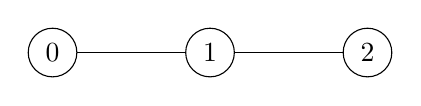
\begin{tikzpicture}
            \node[circle, draw] (1) at (0,0) {0};
            \node[circle, draw] (2) at (2,0) {1};
            \node[circle, draw] (3) at (4,0) {2};
            \draw[-] (1) -- (2);
            \draw[-] (2) -- (3);
        \end{tikzpicture}
        \hspace{1cm}
        $
            \begin{bmatrix}
                0 & 1 & 0 \\
                1 & 0 & 1 \\
                0 & 1 & 0 \\
            \end{bmatrix}
        $
    \end{center}

\end{theorem}

\begin{theorem}
    {Adjacency list}
    An array with $n$ items, each item in the array is a list of nodes that the current node is connected to.

    \begin{itemize}
        \item \textbf{Space:} $O(n+m)$ - better for sparse graphs (less edges).
        \item \textbf{Access (check):} $O(m)$ for determining if there is a connection between two nodes.
        \item \textbf{Access (process)}: Better for sparse graphs as less than $n^2$ elements.
    \end{itemize}

    \tcblower

    \begin{center}
        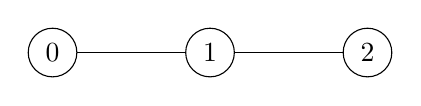
\begin{tikzpicture}
            \node[circle, draw] (1) at (0,0) {0};
            \node[circle, draw] (2) at (2,0) {1};
            \node[circle, draw] (3) at (4,0) {2};
            \draw[-] (1) -- (2);
            \draw[-] (2) -- (3);
        \end{tikzpicture}
        \hspace{1cm}
        $
            [
                    [2],
                    [1,3],
                    [2]
                ]
        $
    \end{center}
\end{theorem}

\begin{theorem}
    {Edge list}
    An array with $m$ items, each item is a tuple of the two nodes that the edge is connecting.
    \tcblower

    \begin{center}
        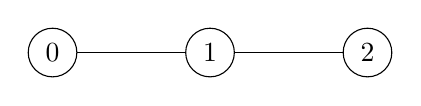
\begin{tikzpicture}
            \node[circle, draw] (1) at (0,0) {0};
            \node[circle, draw] (2) at (2,0) {1};
            \node[circle, draw] (3) at (4,0) {2};
            \draw[-] (1) -- (2);
            \draw[-] (2) -- (3);
        \end{tikzpicture}
        \hspace{1cm}
        $
            [
                    (0,1),
                    (1,2)
                ]
        $
    \end{center}
\end{theorem}

\textbf{Traversal}:

\begin{theorem}
    {Breadth-first search (BFS)}
    Visits nodes at the increasing order of distance from the starting node.
    \begin{itemize}
        \item Queue starting node
        \item Repeat until queue is empty, visit queue node
        \item Add unqueued adjacent nodes to queue and mark as queued.
    \end{itemize}
    \tcblower
    Example implementation: \ref{eg:graph_bfs}
\end{theorem}

\begin{theorem}
    {Depth-first search (DFS)}
    Visit the furthest nodes and backtrack.
\end{theorem}

% \begin{definition}
%     {Dijkstra's algorithm}
%     Finds the shortest path from a starting node to all other nodes in a weighted graph.

% \end{definition}

\subsubsection{Heaps}
\label{subsubsec:heaps}

\begin{theorem}
    {Priority queues}
    A priority queue is a queue where each item has a priority, and the item with the highest priority is accessed / removed first. The most common implementation is the \textbf{heap}.

    \begin{itemize}
        \item \textbf{Access:} $O(1)$ (size, peek)
        \item \textbf{Insertion:} $O(\log n)$ (enqueue, dequeue)
    \end{itemize}
\end{theorem}

\begin{definition}
    {Heap}
    A (max) heap is a binary tree where \underline{each node has a value greater than or equal to its children}. The root node has the highest value.

    \begin{itemize}
        \item \textbf{Max heap}: The root node has the highest value.
        \item \textbf{Min heap}: The root node has the lowest value.
    \end{itemize}

    Thouhg a tree-based data structure, we usually implement heaps as arrays, which is useful such as in the case of \hyperref[def:heapsort]{heap sort}.
\end{definition}

\subsubsection{Trees}

\begin{definition}
    {Trees}
    Nodes which has \textbf{one parent} and can connect to \textbf{multiple children}.
\end{definition}

\begin{knBox}
    {Definitions}
    \begin{itemize}
        \item \textbf{Root}: The top node of the tree.
        \item \textbf{Internal node}: A node with children.
        \item \textbf{Leaf / external node}: A node with no children.
        \item \textbf{Sibilings}: Nodes with the same parent.
        \item \textbf{Height}: The number of edges from the root to the furthest leaf.
        \item \textbf{Depth}: The number of edges from the root to the current node.
              \item\textbf{Sub tree}: A tree that is a child of a node.
        \item \textbf{Degree of node}: The number of immediate children of the node.
        \item \textbf{Degree of tree}: The maximum degree of all nodes.
    \end{itemize}
\end{knBox}

\label{thm:graph_bfs}

\subsubsection{Hash tables}

\begin{definition}
    {Hash table}
    \textbf{Dynamic set} of key-value pairs, where items are stored in an array with \textbf{fixed size}. To access an item, the index is found by a \hyperref[thm:hash-function]{hash function}.

    A \textbf{collision} occurs when $h(k_1) = h(k_2)$. We deal with it by different \hyperref[thm:collision-resolution]{methods}.

    \begin{itemize}
        \item \textbf{Access:} $\Theta(1)$, $O(n)$
        \item \textbf{Insertion \& deletion:} $\Theta(1)$, $O(n)$
    \end{itemize}

    Where $h$ is the hash function and $k$ is the key.

    \textit{Note: Hash tables are a specific implementation of a dictionary. Each item in the hash table table is called a bucket or a slot}
\end{definition}

\begin{knBox}
    {Load factor}
    \[
        \alpha = \frac{n}{m}
    \]
    Where $n$ is the number of items, and $m$ is the size of the table.
\end{knBox}

\begin{theorem}
    {Hash function}
    A hash function is a function that takes a key and returns an index. It should be in relation to the \textbf{size of the table} $m$.

    The most basic hash function is the \textbf{division method}:
    \[
        h(k) = k \% m
    \]
    A good value of $m$ should be a \textbf{prime number} that is not close to a power of 2.
\end{theorem}
\label{thm:hash-function}

\begin{theorem}
    {Collision \& resolution}
    When $h(k_1) = h(k_2)$, we have a \textbf{collision}. We can resolve it by:
    \begin{itemize}
        \item \textbf{Chaining}: Store items in the same slot by \textbf{appending} them to the linked list in the slot.
        \item \textbf{Open addressing}: Store items in another slot.
    \end{itemize}
    For opening addressing, we have the following implementations and the slot where the item is stored is:

    \begin{tabular}{|l|l|}
        \hline
        \textbf{Method}   & \textbf{Slot}             \\
        \hline
        Linear probing    & $A[h(k) + i]$             \\
        Quadratic probing & $A[h(k) + i^2]$           \\
        Double hashing    & $A[h(k) + i \cdot h'(k)]$ \\
        \hline
    \end{tabular}

    Where $i$ is the number of collisions.
\end{theorem}
\label{thm:collision-resolution}

\begin{knBox}
    {Primary clustering}
    Primary clustering occurs in \textbf{open-addressing} hash tables that use \textbf{linear probing} for collision resolution, which can lead to clusters of occupied slots.

    This can lead to \textbf{longer search times} for items that are stored in the same cluster.
\end{knBox}

\begin{theorem}
    {Finding the average number of slots inspected for unsuccessful search}
    General steps:
    \begin{enumerate}
        \item For each slot, assume a collision and resolve until an empty slot is found, and count the steps (no. of slots inspected). We usually count nil slots as well.
        \item Sum and divide by $m$
    \end{enumerate}
    Notes:
    \begin{itemize}
        \item For double hashing, we \textbf{must consider the second hash function}. In other resolution methods, we already assumed a collision so the first hash function does not matter. Refer to example for detailed steps.
    \end{itemize}
    \tcblower
    Example: \ref{eg:hash_unsuccessful_double_hashing}
\end{theorem}
\label{thm:hash_unsuccessful_average_slots_inspected}

\begin{theorem}
    {Average number of slots inspected for successful search}
    General steps:
    \begin{enumerate}
        \item For each slot, count the number of items in the slot.
        \item Sum and divide by $m$
    \end{enumerate}
\end{theorem}

